% !TeX program = xelatex
\documentclass[a4paper,10pt]{article}

% ============================================================================
% សន្លឹកកិច្ចការសិស្ស ស-ខ្មៅ (Student Guided-Inquiry Worksheet - Grade 8 ALG53)
% បរិបទ៖ ថ្នាក់រៀនគ្មានស្លាយ LCD – ២.១-២.៣ សញ្ញាណ ដឺក្រេ និងវិធីបូក-ដកពហុធា (២ ទំព័រ A4)
% ============================================================================
\usepackage[a4paper, left=0.90cm, right=0.90cm, top=0.75cm, bottom=0.85cm, footskip=0.45cm]{geometry}
\usepackage{amsmath, amssymb}
\usepackage{unicode-math}
\usepackage{fontspec}
\usepackage{array, colortbl}
\usepackage[table]{xcolor}
\usepackage{enumitem}
\usepackage{pifont}
\usepackage{fancyhdr}
\usepackage{lastpage}
\usepackage{tikz}
\usepackage[most]{tcolorbox}
\usetikzlibrary{calc, arrows.meta, positioning, babel}

\makeatletter
\let\@expl@@@mark@update@singlecol@structures@@\relax
\makeatother

\providecommand{\NGSFindFonts}{%
  \IfFileExists{C:/Windows/Fonts/cambria.ttc}{%
    \def\NGSSysPath{C:/Windows/Fonts/}%
    \def\NGSUserPath{C:/Users/KIT/AppData/Local/Microsoft/Windows/Fonts/}%
  }{%
    \IfFileExists{./fonts/KhmerOSsiemreap.ttf}{\def\NGSSysPath{./fonts/}\def\NGSUserPath{./fonts/}}{%
    \IfFileExists{../fonts/KhmerOSsiemreap.ttf}{\def\NGSSysPath{../fonts/}\def\NGSUserPath{../fonts/}}{%
    \IfFileExists{../../fonts/KhmerOSsiemreap.ttf}{\def\NGSSysPath{../../fonts/}\def\NGSUserPath{../../fonts/}}{%
    \IfFileExists{../../../fonts/KhmerOSsiemreap.ttf}{\def\NGSSysPath{../../../fonts/}\def\NGSUserPath{../../../fonts/}}{%
    \IfFileExists{../../../../fonts/KhmerOSsiemreap.ttf}{\def\NGSSysPath{../../../../fonts/}\def\NGSUserPath{../../../../fonts/}}{%
    \IfFileExists{../../../../../fonts/KhmerOSsiemreap.ttf}{\def\NGSSysPath{../../../../../fonts/}\def\NGSUserPath{../../../../../fonts/}}{%
    \IfFileExists{../../../../../../fonts/KhmerOSsiemreap.ttf}{\def\NGSSysPath{../../../../../../fonts/}\def\NGSUserPath{../../../../../../fonts/}}{%
      \def\NGSSysPath{../../../../../../../fonts/}\def\NGSUserPath{../../../../../../../fonts/}%
    }}}}}}}%
  }%
}
\NGSFindFonts

\setmathfont[Path={\NGSSysPath}, FontIndex=1, Scale=1.02]{cambria.ttc}
\defaultfontfeatures{Ligatures=TeX}

\setmainfont[
  Path={\NGSUserPath},
  Extension=.ttf,
  Script=Khmer,
  BoldFont={KhmerOSsiemreap},
  BoldFeatures={FakeBold=1.8},
  ItalicFont={KhmerOSsiemreap},
  ItalicFeatures={FakeSlant=0.25},
  BoldItalicFont={KhmerOSsiemreap},
  BoldItalicFeatures={FakeBold=1.8, FakeSlant=0.25}
]{KhmerOSsiemreap}

\newfontfamily\muol[Path={\NGSUserPath}, Extension=.ttf, Script=Khmer]{KhmerOSmuollight}
\newfontfamily\TimesEn[Path={\NGSSysPath}, Extension=.ttf, BoldFont={timesbd}, ItalicFont={timesi}, BoldItalicFont={timesbi}]{times}

\XeTeXlinebreaklocale "km"
\XeTeXlinebreakskip = 0pt plus 1pt minus 0.1pt

\definecolor{panelgray}{gray}{0.94}
\definecolor{headgray}{gray}{0.86}

\pagestyle{fancy}
\fancyhf{}
\renewcommand{\headrulewidth}{0pt}
\fancyfoot[L]{\fontsize{8pt}{10pt}\selectfont អនុវិទ្យាល័យព្រះក្រសាំង \en{|} គណិតវិទ្យា ថ្នាក់ទី៨ \en{|} មេរៀនទី៥ (២.១--២.៣ សញ្ញាណ ដឺក្រេ និងវិធីបូក-ដកពហុធា)}
\fancyfoot[R]{\fontsize{8.2pt}{10pt}\selectfont ទំព័រ \en{\thepage\ / \pageref{LastPage}}}

\setlength{\parindent}{0pt}
\setlength{\parskip}{0pt}
\setlength{\tabcolsep}{4pt}

\newcommand{\en}[1]{{\TimesEn #1}}
\newcommand{\enbf}[1]{{\TimesEn\textbf{#1}}}
\newcommand{\unit}[1]{\,\text{\en{#1}}}
\newcommand{\cnum}[1]{{\fontsize{10pt}{12pt}\selectfont\ding{\numexpr171+#1\relax}}}
\newcommand{\chk}{\tikz[baseline=-0.15ex]\draw[black, line width=0.8pt] (0,0) rectangle (0.25cm,0.25cm);}
\newcommand{\dotline}[1]{\makebox[#1]{\dotfill}}

\newcolumntype{L}[1]{>{\raggedright\arraybackslash}p{#1}}
\newcolumntype{C}[1]{>{\centering\arraybackslash}p{#1}}

\newcommand{\secbar}[2]{%
  \vspace{3pt}
  \noindent\colorbox{headgray}{\parbox{\dimexpr\linewidth-2\fboxsep\relax}{%
    \vspace{1.5pt}{\muol\fontsize{9.5pt}{13.5pt}\selectfont #1}\hfill{\fontsize{8.5pt}{12pt}\selectfont\textbf{#2}}\vspace{1.5pt}%
  }}\par\vspace{3pt}
}

\begin{document}
\fontsize{9.5pt}{14.2pt}\selectfont

% ============================================================================
% ទំព័រទី១៖ ក្បាលសន្លឹកកិច្ចការ + E1 + E2 + E3
% ============================================================================
\begin{tcolorbox}[enhanced, sharp corners, colback=white, colframe=black, boxrule=1.0pt, top=4pt, bottom=4pt, left=6pt, right=6pt]
  \begin{center}
    {\muol\fontsize{10.5pt}{15pt}\selectfont សន្លឹកកិច្ចការសិស្ស — មេរៀនទី៥៖ កន្សោមពីជគណិត \enbf{(}២.១--២.៣ ពហុធា\enbf{)}}\\[2pt]
    {\footnotesize សៀវភៅសិក្សាគោលថ្នាក់ទី៨ ទំព័រ ៥៦--៥៩ \en{|} តារាងតម្រឹមដឺក្រេមានខ្ទង់សូន្យ និងរបាំងសញ្ញាដក (គ្មានស្លាយ \en{LCD})}
  \end{center}
  \vspace{2pt}
  \hrule height 0.5pt
  \vspace{4pt}
  ឈ្មោះសិស្ស៖ \dotline{5.3cm} ថ្នាក់៖ \dotline{2.0cm} ដៃគូទី៖ \dotline{2.0cm} កាលបរិច្ឆេទ៖ \dotline{3.3cm}
\end{tcolorbox}

% -------------------- ផ្នែកទី១៖ E1 ENGAGE --------------------
\secbar{ផ្នែកទី១ ៖ បេសកកម្មភ្ជាប់បញ្ហា \enbf{(E1 — Engage)} — បរិមាត្រត្រីកោណ និងអន្ទាក់ដឺក្រេពហុធា}{\en{3} នាទី (ទស្សន៍ទាយមុនរៀន)}

\begin{tcolorbox}[enhanced, sharp corners, colback=panelgray, colframe=black, boxrule=0.8pt, top=3.5pt, bottom=3.5pt, left=6pt, right=6pt]
  \begin{minipage}[c]{13.4cm}
    ១) ត្រីកោណ $ABC$ (ទំ.៥៦) មានជ្រុង $3y, 2x$ និង $8$ $\implies$ បរិមាត្រស្មើ $AB+BC+CA = \dotline{3.2cm}$ ។\\[2pt]
    ២) \textbf{បេសកកម្មទស្សន៍ទាយ៖} ចំពោះពហុធា $y^3 + 4y^4x + 7 + y$ (ទំ.៥៧) តើដឺក្រេរបស់វាស្មើប៉ុន្មាន?\\[1.5pt]
    \hspace*{0.3cm}\chk\ ស្មើ $4$ (លេខនិទស្សន្តធំជាងគេ) \quad
    \chk\ ស្មើ $5$ (ដឺក្រេតួខ្ពស់បំផុត $4y^4x^1$) \quad
    \chk\ ស្មើ $9$ (បូកដឺក្រេគ្រប់តួ)
  \end{minipage}\hfill
  \begin{minipage}[c]{4.8cm}
    \centering
    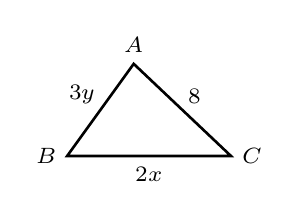
\begin{tikzpicture}[scale=0.65, every node/.style={font=\footnotesize, text=black}]
      \draw[black, line width=0.95pt, fill=white] (1.3,1.8) -- (0,0) -- (3.2,0) -- cycle;
      \node[above=0.5pt] at (1.3,1.8) {$A$};
      \node[left=0.5pt] at (0,0) {$B$};
      \node[right=0.5pt] at (3.2,0) {$C$};
      \node[above left=-2pt] at (0.65,0.9) {$3y$};
      \node[above right=-2pt] at (2.25,0.9) {$8$};
      \node[below=0.5pt] at (1.6,0) {$2x$};
    \end{tikzpicture}
  \end{minipage}
\end{tcolorbox}

% -------------------- ផ្នែកទី២៖ E2 EXPLORE --------------------
\secbar{ផ្នែកទី២ ៖ រុករកសញ្ញាណ ដឺក្រេ និងវិធីបូក-ដកពហុធា \enbf{(E2 — Explore)}}{\en{11} នាទី (ពិភាក្សាដៃគូ)}

\textbf{ក. សកម្មភាពទី១ (ញែកតួ ចំណាត់ថ្នាក់ និងដឺក្រេនៃពហុធា ទំ.៥៦--៥៨)៖}
\begin{enumerate}[label=\arabic*., leftmargin=0.55cm, itemsep=3.5pt, topsep=2pt]
  \item ចូរបំពេញចំនួនតួ និងឈ្មោះពិសេស៖ $3x - 8$ មាន $\dotline{0.9cm}$ តួ ហៅថា \textbf{ទ្វេធា} \;,\; ចំណែក $-2x^3y - 3y + 5$ មាន $\dotline{0.9cm}$ តួគឺ $-2x^3y$, \dotline{1.4cm} និង \dotline{1.2cm} ហៅថា \textbf{ត្រីធា} ។
  \item \textbf{អន្ទាក់មិនមែនពហុធា (ទំ.៥៧)៖} ហេតុអ្វីកន្សោម $x + \dfrac{3}{b^2}$ \textbf{មិនមែនជាពហុធា}? ព្រោះតួ $\dfrac{3}{b^2}$ \dotline{4.8cm} ។
  \item \textbf{រកដឺក្រេនៃពហុធា $y^3 + 4y^4x + 7 + y$៖} ដឺក្រេនៃតួទី១ $(y^3)$ គឺ $3$ \;;\; តួទី២ $(4y^4x^1)$ គឺ $4+\dotline{0.8cm}=\dotline{0.9cm}$ \;;\; តួទី៣ $(7)$ គឺ $\dotline{0.8cm}$ \;;\; តួទី៤ $(y^1)$ គឺ $\dotline{0.8cm}$ ។ ដូចនេះ ដឺក្រេខ្ពស់ជាងគេគឺ $\dotline{1.2cm}$ ។
\end{enumerate}

\vspace{4pt}
\textbf{ខ. សកម្មភាពទី២ (វិធីបូក និងដកពហុធាតាមជួរដេក ទំ.៥៨ និងតាមជួរឈរមានខ្ទង់ $0x$ ទំ.៥៩)៖}
\begin{enumerate}[label=\arabic*., leftmargin=0.55cm, itemsep=4pt, topsep=2pt]
  \item \textbf{បូកតាមជួរដេក (ផ្ដុំឯកធាដូចគ្នា ទំ.៥៨)៖} គេឱ្យ $A = 2a^2 + 3a - 4$ និង $B = 5a^2 - 7a + 6$ ៖\\
  $A + B = (2a^2 + 5a^2) + (3a - 7a) + (-4 + 6) = \dotline{4.5cm}$ ។
  \item \textbf{ដកតាមជួរដេក (របាំងសញ្ញាដកមុខវង់ក្រចក ទំ.៥៨)៖} គេឱ្យ $E = 3x^2 - 2x + 7$ និង $F = x^2 + 4x + 5$ ៖\\
  $E - F = (3x^2 - 2x + 7) - (x^2 + 4x + 5) = 3x^2 - 2x + 7 - x^2 \dotline{1.5cm} \dotline{1.5cm} = \dotline{3.8cm}$ ។
  \item \textbf{តាមជួរឈរ (ខ្ទង់បាត់ត្រូវដាក់ $0x$ ទំ.៥៩)៖} គេឱ្យ $A = 5x^3 - 2x^2 + 7x + 4$ និង $B = 2x^3 + 4x^2 - 6$ ៖\\[3pt]
  \begin{minipage}[t]{8.8cm}
    \centering
    \begin{tabular}{r@{\;}r@{\;}r@{\;}r@{\;}r}
      & $5x^3$ & $-\,2x^2$ & $+\,7x$ & $+\,4$ \\
      $+$ & $2x^3$ & $+\,4x^2$ & $+\,\mathbf{0x}$ & $-\,6$ \\
      \hline
      $A+B =$ & \dotline{1.3cm} & \dotline{1.5cm} & \dotline{1.4cm} & \dotline{1.3cm}
    \end{tabular}
  \end{minipage}\hfill
  \begin{minipage}[t]{8.8cm}
    \centering
    \begin{tabular}{r@{\;}r@{\;}r@{\;}r@{\;}r}
      & $5x^3$ & $-\,2x^2$ & $+\,7x$ & $+\,4$ \\
      $-$ & $(2x^3$ & $+\,4x^2$ & $+\,\mathbf{0x}$ & $-\,6)$ \\
      \hline
      $A-B =$ & \dotline{1.3cm} & \dotline{1.5cm} & \dotline{1.4cm} & \dotline{1.3cm}
    \end{tabular}
  \end{minipage}
\end{enumerate}

% -------------------- ផ្នែកទី៣៖ E3 EXPLAIN --------------------
\secbar{ផ្នែកទី៣ ៖ សង្ខេបនិយមន័យ និងធនាគារហេតុផល \enbf{(E3 — Explain)}}{\en{6} នាទី (កត់ត្រាខ្លឹមសារគោល)}

\begin{tcolorbox}[enhanced, sharp corners, colback=white, colframe=black, boxrule=0.85pt, top=4pt, bottom=4pt, left=6pt, right=6pt]
  \cnum{1} \textbf{និយមន័យពហុធា (ទំ.៥៧)៖} ពហុធាជាផលបូកនៃពីរ ឬច្រើន \dotline{2.4cm} មិនដូចគ្នា (មាន ២ តួហៅថា \dotline{1.8cm}, មាន ៣ តួហៅថា \dotline{1.8cm}) ។\\[3.5pt]
  \cnum{2} \textbf{ដឺក្រេនៃពហុធា (ទំ.៥៧)៖} គឺជាដឺក្រេរបស់តួដែលមានដឺក្រេ \dotline{2.8cm} (\textbf{ហាម}បូកដឺក្រេគ្រប់តួបញ្ចូលគ្នា!) ។ \cnum{3} អាចរៀបតាម \textbf{លំដាប់កើន} ឬ \textbf{លំដាប់ចុះ} ។\\[3.5pt]
  \cnum{4} \textbf{វិធីបូក និងដកពហុធា (ទំ.៥៨--៥៩)៖} ត្រូវបូក ឬដកតែ \textbf{ឯកធា \dotline{2.2cm}} ។ \cnum{5} មុខវង់ក្រចកមានសញ្ញាដក $(-)$ ត្រូវ \textbf{\dotline{2.2cm} គ្រប់តួ} ក្នុងវង់ក្រចក ហើយពេលសរសេរជួរឈរត្រូវដាក់ខ្ទង់ $\mathbf{0x^k}$ ត្រង់ដឺក្រេដែលបាត់ ។\\[4pt]
  \centering
  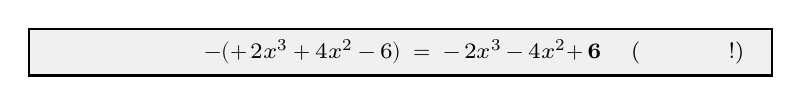
\begin{tikzpicture}
    \node[draw=black, line width=0.8pt, fill=panelgray, inner xsep=10pt, inner ysep=4pt, font=\footnotesize] {របាំងការពារសញ្ញាដក៖ \quad $-(+\,2x^3 + 4x^2 - 6) \;=\; -\,2x^3 - 4x^2 \mathbf{+\,6}$ \quad (ដកប៉ះដកបាន \textbf{បូក}!)};
  \end{tikzpicture}
\end{tcolorbox}

\newpage
% ============================================================================
% ទំព័រទី២៖ E4 (លំហាត់គំរូ ទំ.៥៧-៥៩) + E5 (ប្រតិបត្តិ + Exit Check) + កិច្ចការផ្ទះ
% ============================================================================

% -------------------- ផ្នែកទី៤៖ E4 ELABORATE --------------------
\secbar{ផ្នែកទី៤ ៖ អនុវត្តលំហាត់គំរូតាមសៀវភៅគោល \enbf{(E4 — Elaborate)}}{\en{10} នាទី (បំពេញតាមគំរូ)}

\textbf{១. លំហាត់គំរូទី១ (តារាងដឺក្រេ និងការរៀបលំដាប់កើន-ចុះ ទំ.៥៧--៥៨)៖} ចូរបំពេញតារាងខាងក្រោម៖

\vspace{2pt}
{\renewcommand{\arraystretch}{1.40}
\begin{tabular}{|L{3.8cm}|C{1.8cm}|C{1.6cm}|L{5.2cm}|L{5.2cm}|}
\hline
\cellcolor{headgray}\textbf{ពហុធា} & \cellcolor{headgray}\textbf{អថេរ} & \cellcolor{headgray}\textbf{ដឺក្រេ} & \cellcolor{headgray}\textbf{រៀបតាមលំដាប់កើន} & \cellcolor{headgray}\textbf{រៀបតាមលំដាប់ចុះ} \\
\hline
$11 + 5x^2 - 3x$ & $x$ & $\mathbf{2}$ & $11 - 3x + 5x^2$ & $5x^2 - 3x + 11$ \\
\hline
$2k^3 - 4 + k^2 - k$ & \dotline{1.2cm} & \dotline{1.1cm} & \dotline{4.6cm} & \dotline{4.6cm} \\
\hline
$y^3 + 4y^4x + 7 + y$ & \dotline{1.2cm} & \dotline{1.1cm} & $7 + y + y^3 + 4y^4x$ & \dotline{4.6cm} \\
\hline
\end{tabular}}

\vspace{4pt}
\textbf{២. លំហាត់គំរូទី២ (ផ្ទៀងផ្ទាត់សញ្ញាក្នុងការដកពហុធា)៖}
\begin{itemize}[leftmargin=0.5cm, itemsep=3pt, topsep=2pt]
  \item ចំពោះផលដក $A - B$ ក្នុងផ្នែកទី២ (ខ)៖ ហេតុអ្វីខ្ទង់ចំនួនថេរចុងក្រោយស្មើ $+10$ មិនមែន $-2$?\\
  ចម្លើយ៖ ព្រោះ $4 - (-6) = 4 + \dotline{1.2cm} = \dotline{1.4cm}$ (\cnum{5}) ។
  \item \textbf{សំណួរឆ្លុះបញ្ចាំង (\en{Looking Back})៖} ប្រសិនបើ $A - B = 3x^3 - 6x^2 + 7x + 10$ តើយើងអាចទាញរក $B - A$ ភ្លាមដោយគ្រាន់តែដូរសញ្ញាគ្រប់តួបានឬទេ? គេបាន $B - A = -(A - B) = \dotline{5.5cm}$ ។
\end{itemize}

% -------------------- ផ្នែកទី៥៖ E5 EVALUATE --------------------
\secbar{ផ្នែកទី៥ ៖ ហ្វឹកហាត់ «ប្រតិបត្តិ» និងតេស្តរហ័ស \enbf{(E5 — Evaluate)}}{\en{10} នាទី (ធ្វើដោយខ្លួនឯង រួចប្ដូរផ្ទៀង)}

\textbf{១. ប្រតិបត្តិកំណត់អថេរ ចំនួនតួ (ទំ.៥៧) និងដឺក្រេពហុធា (ទំ.៥៨)៖}

\vspace{2pt}
{\renewcommand{\arraystretch}{1.38}
\begin{tabular}{|L{4.8cm}|L{4.1cm}||L{4.8cm}|L{4.1cm}|}
\hline
\cellcolor{headgray}\textbf{ពហុធា (ទំ.៥៧)} & \cellcolor{headgray}\textbf{អថេរ និងចំនួនតួ} & \cellcolor{headgray}\textbf{ពហុធា (ទំ.៥៨)} & \cellcolor{headgray}\textbf{ដឺក្រេនៃពហុធា} \\
\hline
ក. $6x^3 + 2xy - 4$ & អថេរ \dotline{1.0cm}, \dotline{0.8cm} តួ & ក. $x^2 + x - 3$ & ដឺក្រេ $= \dotline{1.5cm}$ \\
\hline
ខ. $\sqrt{3}ab + 3x + 3$ & អថេរ \dotline{1.0cm}, \dotline{0.8cm} តួ & ខ. $-\dfrac{3}{4}x + 3$ & ដឺក្រេ $= \dotline{1.5cm}$ \\
\hline
គ. $-3x^2y + \dfrac{1}{2}y - 2$ & អថេរ \dotline{1.0cm}, \dotline{0.8cm} តួ & គ. $a^2 + 2ab + c^2d$ & ដឺក្រេ $= \dotline{1.5cm}$ \\
\hline
គំរូ៖ $\dfrac{1}{2}x^2 - 3a + 4$ & អថេរ \dotline{1.0cm}, \dotline{0.8cm} តួ & ឃ. $\sqrt{2}x^2 - 4x$ & ដឺក្រេ $= \dotline{1.5cm}$ \\
\hline
\end{tabular}}

\vspace{4pt}
\textbf{២. ប្រតិបត្តិគណនា $M + N$ និង $M - N$ ទាំង ៣ លំហាត់ (សៀវភៅគោល ទំ.៥៩)៖}
\begin{itemize}[leftmargin=0.5cm, itemsep=3.5pt, topsep=2pt]
  \item ក) គេឱ្យ $M = 2x^2 + 3x + 1$ និង $N = -x^2 + 2x + 4$ ៖\\[1.5pt]
  $M + N = \dotline{7.2cm}$ \qquad;\qquad $M - N = \dotline{7.2cm}$
  \item ខ) គេឱ្យ $M = 12a^2 + 2ab + 54$ និង $N = 9a^2 - 4ab - 25$ ៖\\[1.5pt]
  $M + N = \dotline{7.2cm}$ \qquad;\qquad $M - N = \dotline{7.2cm}$
  \item គ) គេឱ្យ $M = \dfrac{1}{2}xy^2 + 2xy - 3$ និង $N = \dfrac{3}{2}xy^2 - 12xy - 16$ ៖\\[1.5pt]
  $M + N = \dotline{7.2cm}$ \qquad;\qquad $M - N = \dotline{7.2cm}$
\end{itemize}

\vspace{4pt}
\begin{tcolorbox}[enhanced, sharp corners, colback=panelgray, colframe=black, boxrule=0.85pt, top=3pt, bottom=3pt, left=6pt, right=6pt]
  \textbf{៣. បិទបេសកកម្ម \en{E1} និងតេស្តរហ័ស (\en{Exit Check — 60} វិនាទី)៖}\\[2pt]
  $\bullet$ \textbf{ចម្លើយបេសកកម្ម \en{E1}៖} ពហុធា $y^3 + 4y^4x + 7 + y$ មានដឺក្រេស្មើ $\dotline{1.5cm}$ (យកពីតួខ្ពស់បំផុត $4y^4x^1$) ។\\[2pt]
  $\bullet$ \textbf{សំណួរតេស្តរហ័ស៖} បើ $P = 4x^2 - 3x + 2$ និង $Q = x^2 - 3x - 5$ តើផលដក $P - Q$ ស្មើប៉ុន្មាន?\\[1.5pt]
  \hspace*{0.3cm}\enbf{A.}\; $3x^2 - 6x - 3$ \qquad\quad
  \enbf{B.}\; $3x^2 - 3$ \qquad\quad
  \enbf{C.}\; $3x^2 + 7$ \qquad\quad
  \enbf{D.}\; $5x^2 - 6x + 7$
\end{tcolorbox}

% -------------------- ផ្នែកទី៦៖ កិច្ចការផ្ទះ --------------------
\secbar{ផ្នែកទី៦ ៖ ប័ណ្ណកិច្ចការផ្ទះ \enbf{(Homework)} និងការអានជាមុន}{សៀវភៅសិក្សាគោល ទំ.៧២--៧៣}

\begin{tcolorbox}[enhanced, sharp corners, colback=white, colframe=black, boxrule=0.8pt, borderline={0.6pt}{2pt}{dashed}, top=3pt, bottom=3pt, left=6pt, right=6pt]
  \textbf{១. លំហាត់ទី២ (ទំ.៧២)៖} សរសេរចំនួនគត់ $1997,\; 2674,\; 20011$ ជាពហុធារៀបតាមលំដាប់ចុះដឺក្រេនៃ $10$ ។\\[1.5pt]
  \textbf{២. លំហាត់ទី៤ (ទំ.៧២)៖} គេមាន $A = 2x^2 + x^4 - 3x + 1$ និង $B = x^2 - 3x^3 - 2x^4 - x + 3$ ។ គណនា $A - B$ (រៀបដឺក្រេចុះ) និង $B - A$ ។\\[1.5pt]
  \textbf{៣. លំហាត់ទី៥ ខ--គ (ទំ.៧៣)៖} គណនាផលបូក៖ $(5a^3b^2-3ab) + (2a^3b^2-ab)$ និង $(4x^4-3y^3+z) + (3x^3+2y^2-4z)$ ។\\[1.5pt]
  $\bullet$ \textbf{អានជាមុន៖} ចំណុច \textbf{២.៤ វិធីគុណពហុធា និង ២.៥ វិធីចែកពហុធា} (សៀវភៅគោល ទំព័រ ៥៩--៦២) ។
\end{tcolorbox}

\end{document}
